The following is a PD control system for a hydraulic actuator.

\begin{center}
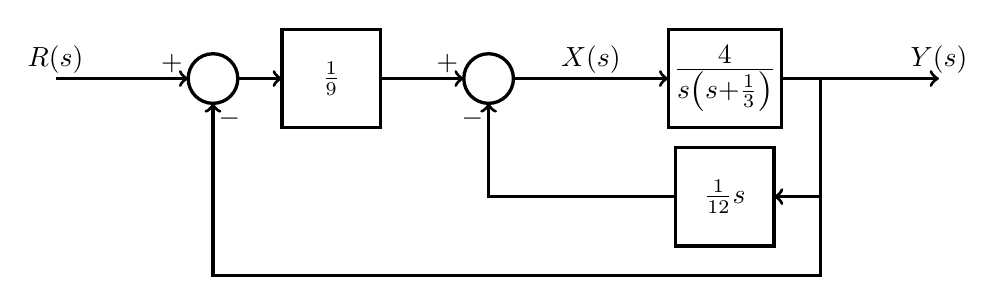
\begin{tikzpicture}[scale=1,inner sep=0pt,outer sep=0pt,very thick,
sysblock/.style={draw,rectangle,inner sep=2pt,minimum width=1.25cm,minimum height=1.25cm,very thick}]
\draw (2,0) node[draw,circle] (sum1) {$\rule{0pt}{18pt}$};
\draw (3.5,0) node[sysblock] (Kp) { $\frac{1}{9}$};
\draw (5.5,0) node[draw,circle] (sum2) {$\rule{0pt}{18pt}$};
\draw (8.5,0) node[sysblock] (G) {\Large $\frac{4}{s\left(s+\frac{1}{3}\right)}$};
\draw (8.5,-1.5) node[sysblock] (Kd) {$\frac{1}{12}s$};
\draw[->] (0,0) node[above=2pt] {$R(s)$} -- (sum1.180) node[above left=2pt] {$+$};
\draw[->] (sum1.0) --  (Kp);
\draw[->] (Kp) -- (sum2.180) node[above left=2pt] {$+$};
\draw[->] (sum2.0) -- node[pos=.5,above=2pt] {$X(s)$} (G.180);
\draw[->] (G.0) -- ++(2,0) node[above=2pt] {$Y(s)$};
\draw[->] (G.0) ++(0.5,0) |- (Kd.0);
\draw[->] (Kd.180) -| (sum2.-90) node[below left=2pt] {$-$};
\draw[->] (G.0) ++(0.5,0) -- ++(0,-2.5) -| (sum1.-90) node[below right=2pt] {$-$};
\end{tikzpicture}
\end{center}

A unit step reference command $r(t)=u(t)$ is applied. Which of the following is a plot of the output $y(t)$? \begin{center}
\includegraphics[width=6in]{\mainfolder/LectureNotes/\lecturefolder/HomeworkProblems/Problem06/prob3}
\end{center}
